\documentclass[11pt,a4paper]{article}

% Packages for formatting and graphics
\usepackage[utf8]{inputenc}
\usepackage{geometry}
\usepackage{graphicx}
\usepackage{listings}
\usepackage{xcolor}

% Page geometry
\geometry{margin=2.5cm}

% R code styling
\definecolor{codegreen}{rgb}{0,0.6,0}
\definecolor{codegray}{rgb}{0.5,0.5,0.5}
\definecolor{codepurple}{rgb}{0.58,0,0.82}
\definecolor{backcolour}{rgb}{0.95,0.95,0.92}

\lstdefinestyle{rstyle}{
    backgroundcolor=\color{backcolour},   
    commentstyle=\color{codegreen},
    keywordstyle=\color{magenta},
    numberstyle=\tiny\color{codegray},
    stringstyle=\color{codepurple},
    basicstyle=\ttfamily\footnotesize,
    breakatwhitespace=false,         
    breaklines=true,                 
    captionpos=b,                    
    keepspaces=true,                 
    numbers=none,                    
    showspaces=false,                
    showstringspaces=false,
    showtabs=false,                  
    tabsize=2,
    frame=single,
    rulecolor=\color{blue!30!black}
}

\lstset{style=rstyle}

\begin{document}

\begin{lstlisting}[language=R]
library(ggplot2)
library(readxl)

setwd("/home/vicente/projeto-pe-2024-2025")

# Read data
wine_data_raw <- read_excel("wine_prod_EU.xlsx")

# Filter and clean data for 2003
wine_data_filtered <- wine_data_raw[!is.na(wine_data_raw$Category) & 
                                   wine_data_raw$`Product Group` != "Non-Vinified" & 
                                   wine_data_raw$Year == 2003, ]

# Create Country_Group variable
wine_data_filtered$Country_Group <- ifelse(wine_data_filtered$`Member State` %in% c("France", "Italy", "Spain"), 
                                           wine_data_filtered$`Member State`, "Others")

# Aggregate data by Country_Group and Category
wine_data <- aggregate(Availability ~ Country_Group + Category, 
                      data = wine_data_filtered, 
                      FUN = sum, na.rm = TRUE)
names(wine_data)[3] <- "Total_Availability"

# Create bar chart
plot <- ggplot(wine_data, aes(x = Category, y = Total_Availability, fill = Country_Group)) +
  geom_bar(stat = "identity", position = "dodge") +
  labs(title = "Wine Availability by Category and Country Group in 2003",
       x = "Wine Category", y = "Availability (10^3 hL)", fill = "Country Group") +
  theme_minimal() +
  theme(axis.text.x = element_text(angle = 45, hjust = 1)) +
  scale_fill_brewer(type = "qual", palette = "Set2")
\end{lstlisting}

\begin{figure}[htbp]
    \centering
    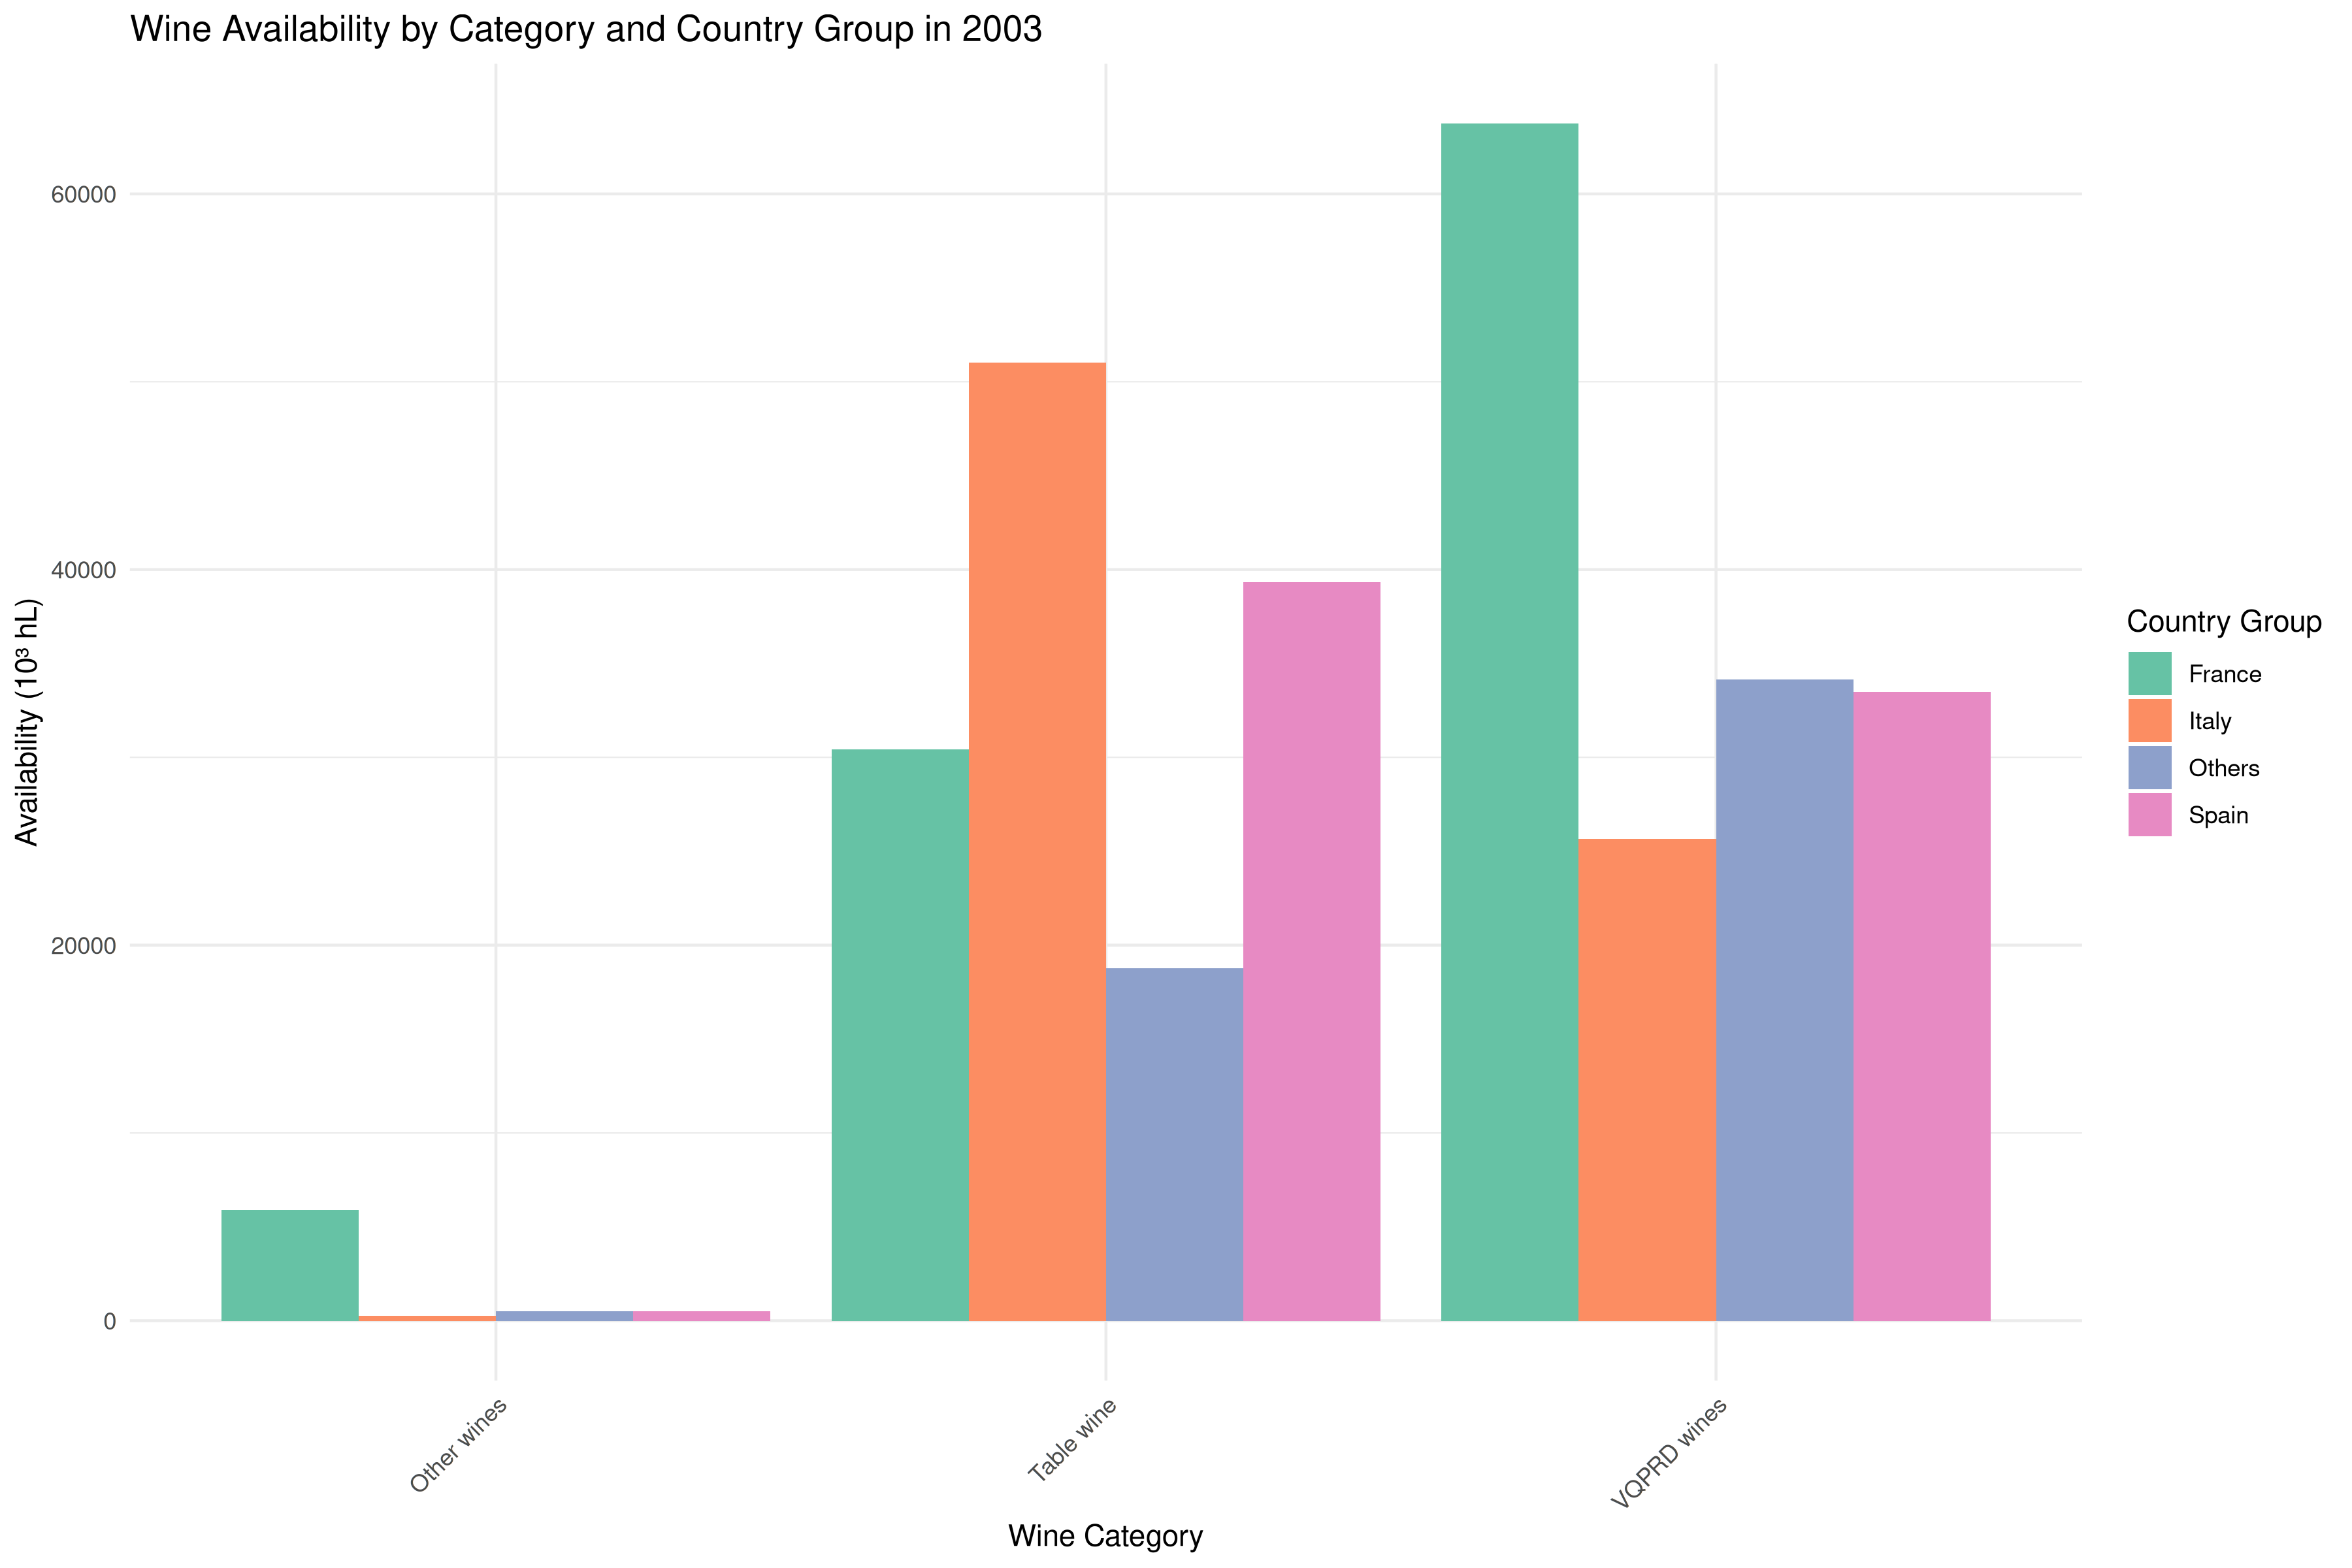
\includegraphics[width=0.9\textwidth]{wine_availability_2003.png}
\end{figure}

\end{document}
